%!TEX root = ../../thesis.tex

\ac{ggF} is modelled by \meps{\powhegbox}{\pythia{8}}, including the exact mass 
dependence of the \Ptop and \Pbottom quarks in the loop \cite{Powheg-ggF-quarkmasses}. 
The CT10 PDF \cite{CTEQ} was used to model the incoming partons.
The \powhegbox parameter \verb|hfact| controls the scale at which the emission 
transitions from Sudakov-like to ME-like. This is tuned to $\mH/1.2$ in order to 
reproduce the Higgs boson \pt distribution of \hqt \cite{HqT2} (NLO+NNLL accuracy). This 
tuning is further discussed in \Section~4.9 of \Reference \cite{YR2}.



\subsection{Higgs boson transverse momentum}
\todo[inline]{Include Higgs \pt studies?}



\subsection{Event selection acceptance}

In \Section~\ref{sec:ggf_jetbin}, perturbative uncertainties in the jet binning were 
considered. We now consider uncertainties in the acceptance of the event selection. These 
are evaluated at hadron-level (\ie before detector simulation) by changing some aspect of 
the MC modelling and measuring the effect upon the acceptance within each jet bin. 
The selection criteria are similar to those applied at detector-level (see 
\Table~\ref{tab:signal:acc_truthselection}).

Hadron-level object definitions follow. The MC event record is used to identify leptons 
and neutrinos which descend from the Higgs boson. An \metvec vector is constructed from 
the neutrinos. Each lepton is `dressed' with the four-momenta of photons within a cone of 
$\Delta R < 0.1$, in order to recover energy lost via QED FSR. Jets are found using 
individual particles as inputs (\cf topo-clusters at detector-level). Muons and neutrinos 
are excluded from jet finding since they interact weakly with the calorimeter. Objects 
must pass the same \pt, $\eta$ and overlap removal criteria applied at detector-level.

\begin{table}
	\begin{tabular}{ccc}
		Jet binning & \ee/\mm & \em/\me \\
		\hline
		Inclusive & \multicolumn{2}{c}{Exactly 2 opposite-sign leptons} \\
		& \multicolumn{2}{c}{\unit{$\ptleadlep > 22$}{\GeV}} \\
		& \unit{$\mll > 12$}{\GeV} & \unit{$\mll > 10$}{\GeV} \\
		& \unit{$\mods{\mll - \mZ} > 15$}{\GeV} & -- \\
		\hline
		0-jet & \unit{$\metrel > 40$}{\GeV} & \unit{$\met > 20$}{\GeV} \\
		& \multicolumn{2}{c}{$\dphillmet > 1.57$} \\
		& \multicolumn{2}{c}{\unit{$\ptll > 30$}{\GeV}} \\
		& \multicolumn{2}{c}{\unit{$\mll < 55$}{\GeV}} \\
		& \multicolumn{2}{c}{$\dphill < 1.8$} \\
		\hline
		1-jet & \unit{$\metrel > 40$}{\GeV} & \unit{$\met > 10$}{\GeV} \\
		& -- & \unit{$\maxmtw > 50$}{\GeV} \\
		& -- & \unit{$\mtautau < 66$}{\GeV} \\
		& \multicolumn{2}{c}{\unit{$\mll < 55$}{\GeV}} \\
		& \multicolumn{2}{c}{$\dphill < 1.8$} \\
		\hline
		\twojet & \unit{$\met > 45$}{\GeV} & \unit{$\met > 20$}{\GeV} \\
		& \multicolumn{2}{c}{\unit{$\mtautau < 66$}{\GeV}} \\
		& \multicolumn{2}{c}{Fails $\dyjj > 3.6$ or \unit{$\mjj > 600$}{\GeV} or CJV or OLV} \\
		& \multicolumn{2}{c}{\unit{$\mll < 55$}{\GeV}} \\
		& \multicolumn{2}{c}{$\dphill < 1.8$} \\
	\end{tabular}
	\caption{Hadron-level event selection used to calculate ggF acceptance uncertainties. 
	The CJV and OLV are the central jet veto and outside lepton veto, respectively. See 
	\Chapter~\ref{chap:selection} for a detailed explanation of the criteria.}
	\label{tab:signal:acc_truthselection}
\end{table}

Four sources of theoretical uncertainty are considered:
\begin{itemize}[noitemsep,nolistsep]
	\item higher order corrections,
	\item \acp{PDF},
	\item parton shower, hadronisation and underlying event models,
	\item NLO-PS matching scheme.
\end{itemize}

Uncertainties due to higher order corrections are evaluated via independent variation of 
renormalisation and factorisation scales in the range $\mH/2 \leq \mur,\muf \leq 2\mH$, 
whilst observing the constraint $1/2 \leq \mur/\muf \leq 2$. In the \twojet bin, scale 
uncertainties are evaluated \todo{H+2j scale uncertainties in acceptance} with \mcfm 
\cite{MCFM:H2j}. This is necessary because \powhegbox is an NLO generator and therefore 
cannot probe perturbative uncertainties in the \twojet bin.

Uncertainties due to \acp{PDF} are evaluated in two ways. The acceptance is compared to 
that predicted with the MSTW2008 PDF \cite{MSTW}. Also, the set of PDF eigenvectors 
corresponding to 90\% \ac{CL} of the CT10 fit were used to evaluate an uncertainty, 
which was then rescaled to 68\% \ac{CL}. PDF uncertainties are calculated relative to the 
inclusive cross section, in order to include uncertainties in the jet binning.

Uncertainties due to the \ac{PS}, hadronisation and \ac{UE} models are evaluated by 
comparing \powhegbox showered by \pythia{8} (nominal), \pythia{6} and \fherwig. 
Uncertainties due to the NLO-PS matching scheme are evaluated by comparing 
\meps{\powhegbox}{\fherwig} to \meps{\mcatnlo}{\herwigpp}.

The uncertainties in each signal region are shown in 
\Table~\ref{tab:signal:acc_unc_summary}. In the fitting procedure, the signal regions are 
further split into bins of \ptsubleadlep and \mll in order to exploit the different 
background compositions. The uncertainties in these split signal regions are shown in 
\Table~\ref{tab:signal:acc_unc_binned}.

\begin{table}[b]
	\begin{tabular}{r|ccccccc|c}
		& \multirow{2}{*}{Stat.} & \multirow{2}{*}{Scale} & \multicolumn{2}{c}{PDF} & \multicolumn{2}{c}{PS/Had./UE} & \multirow{2}{*}{NLO-PS} & \multirow{2}{*}{Total} \\
		& & & MSTW & 68\% CL & \pythia{6} & \fherwig & & \\
		\hline
		\multicolumn{9}{c}{\ee/\mm channels} \\
		\hline
		0-jet   & 0.6\% & 1.4\% & +1.9\% & 3.2\% & $+1.6\%$ & $+6.4\%$ & $-2.5\%$ & 8.1\% \\
		1-jet   & 1.0\% & 1.9\% & +1.8\% & 2.8\% & $-0.7\%$ & $+2.1\%$ & $-1.1\%$ & 4.6\% \\
		\twojet & 1.5\% &       & +2.0\% & 2.3\% & $+0.8\%$ & $-1.0\%$ & $-6.3\%$ &  \\
		\hline
		\multicolumn{9}{c}{\em/\me channels} \\
		\hline
		0-jet   & 0.5\% & 1.1\% & +1.9\% & 3.2\% & $-0.5\%$ & $+2.2\%$ & $-1.8\%$ & 4.8\% \\
		1-jet   & 0.8\% & 1.3\% & +1.8\% & 2.8\% & $+0.5\%$ & $+3.5\%$ & $-1.1\%$ & 5.1\% \\
		\twojet & 1.2\% &       & +2.0\% & 2.2\% & $-0.5\%$ & $+1.5\%$ & $-4.5\%$ &  \\
	\end{tabular}
	\caption{Theoretical uncertainties in the ggF acceptance for each signal region. PDF 
	uncertainties are relative to the inclusive cross section, whereas others are 
	calculated within jet bins. Statistical uncertainties are shown for reference.}
	\label{tab:signal:acc_unc_summary}
\end{table}

\begin{table}
	\centering
	\begin{tabular}{ccc|cccccc}
		& \ptsubleadlep & \mll & \multirow{2}{*}{Scale} & \multicolumn{2}{c}{PDF} & \multicolumn{2}{c}{PS/Had./UE} & \multirow{2}{*}{NLO-PS} \\
		& (\GeV) & (\GeV) & & MSTW & 68\% CL & \pythia{6} & \fherwig & \\
		\hline
		\multicolumn{9}{c}{\ee/\mm channels} \\
		\hline
		\multirow{2}{*}{0-jet}
		&  $>10$ & 12--30 & 2.5\% & +1.9\% & 3.2\% & $+1.8\%$ & $+7.2\%$ & $-4.2\%$ \\
		&  $>10$ & 30--55 & 1.1\% & +1.9\% & 3.3\% & $+1.3\%$ & $+5.6\%$ & $-0.6\%$ \\
		\hline
		\multirow{2}{*}{1-jet}
		&  $>10$ & 12--30 & 2.5\% & +1.8\% & 2.7\% & $-0.5\%$ & $+3.9\%$ & $-3.0\%$ \\
		&  $>10$ & 30--55 & 1.2\% & +1.8\% & 2.8\% & $-0.9\%$ & $+0.2\%$ & $+1.1\%$ \\
		\hline
		\multirow{2}{*}{\twojet}
		&  $>10$ & 12--30 &       & +2.0\% & 2.2\% & $+2.9\%$ & $-0.6\%$ & $-6.5\%$ \\
		&  $>10$ & 30--55 &       & +2.1\% & 2.3\% & $-1.8\%$ & $-1.4\%$ & $-6.1\%$ \\
		\hline
		\multicolumn{9}{c}{\em/\me channels} \\
		\hline
		\multirow{6}{*}{0-jet}
	    & 10--15 & 10--30 & 2.6\% & +1.8\% & 3.2\% & $-1.7\%$ & $+5.7\%$ & $-3.5\%$ \\
		& 15--20 & 10--30 & 1.3\% & +1.9\% & 3.2\% & $+2.2\%$ & $+4.9\%$ & $-2.8\%$ \\
		&  $>20$ & 10--30 & 1.0\% & +1.9\% & 3.2\% & $-2.2\%$ & $-0.6\%$ & $-0.5\%$ \\
		& 10--15 & 30--55 & 1.5\% & +1.8\% & 3.3\% & $+0.8\%$ & $+5.5\%$ & $-3.8\%$ \\
		& 15--20 & 30--55 & 1.5\% & +1.9\% & 3.3\% & $-0.1\%$ & $+2.0\%$ & $-2.5\%$ \\
		&  $>20$ & 30--55 & 3.5\% & +1.9\% & 3.3\% & $-1.9\%$ & $-2.4\%$ & $<0.1\%$ \\
		\hline
		\multirow{6}{*}{1-jet}
	    & 10--15 & 10--30 & 3.2\% & +1.7\% & 2.9\% & $+2.1\%$ & $+11\%$  & $-4.4\%$ \\
		& 15--20 & 10--30 & 2.9\% & +1.8\% & 2.9\% & $+0.8\%$ & $+1.8\%$ & $+1.7\%$ \\
		&  $>20$ & 10--30 & 3.5\% & +1.8\% & 2.7\% & $<0.1\%$ & $+0.4\%$ & $-0.3\%$ \\
		& 10--15 & 30--55 & 5.8\% & +1.7\% & 3.0\% & $+1.2\%$ & $+11\%$  & $-6.2\%$ \\
		& 15--20 & 30--55 & 1.0\% & +1.8\% & 3.3\% & $+2.5\%$ & $+13\%$  & $+6.7\%$  \\
		&  $>20$ & 30--55 & 1.3\% & +1.8\% & 2.8\% & $-0.7\%$ & $-2.1\%$ & $<0.1\%$ \\
		\hline
		\multirow{6}{*}{\twojet}
	    & 10--15 & 10--30 &       & +2.0\% & 2.3\% & $+0.8\%$ & $+14\%$  & $-9.8\%$ \\
		& 15--20 & 10--30 &       & +2.0\% & 2.3\% & $+5.7\%$ & $+23\%$  & $-3.5\%$  \\
		&  $>20$ & 10--30 &       & +2.0\% & 2.2\% & $-0.8\%$ & $-4.7\%$ & $-4.7\%$ \\
		& 10--15 & 30--55 &       & +1.9\% & 2.3\% & $-5.9\%$ & $+1.0\%$ & $+8.2\%$ \\
		& 15--20 & 30--55 &       & +2.0\% & 2.3\% & $-6.6\%$ & $+0.5\%$ & $-1.4\%$ \\
		&  $>20$ & 30--55 &       & +1.9\% & 2.2\% & $+0.3\%$ & $-0.9\%$ & $-5.2\%$ \\
	\end{tabular}
	\caption{Theoretical uncertainties in the ggF acceptance for each signal region, 
	split into bins of \ptsubleadlep and \mll as used in the fitting procedure. PDF 
	uncertainties are relative to the inclusive cross section, whereas others are 
	calculated within jet bins.}
	\label{tab:signal:acc_unc_binned}
\end{table}





\subsection{\mt shape modelling}



\subsection{ME-PS matching}

\begin{figure}
	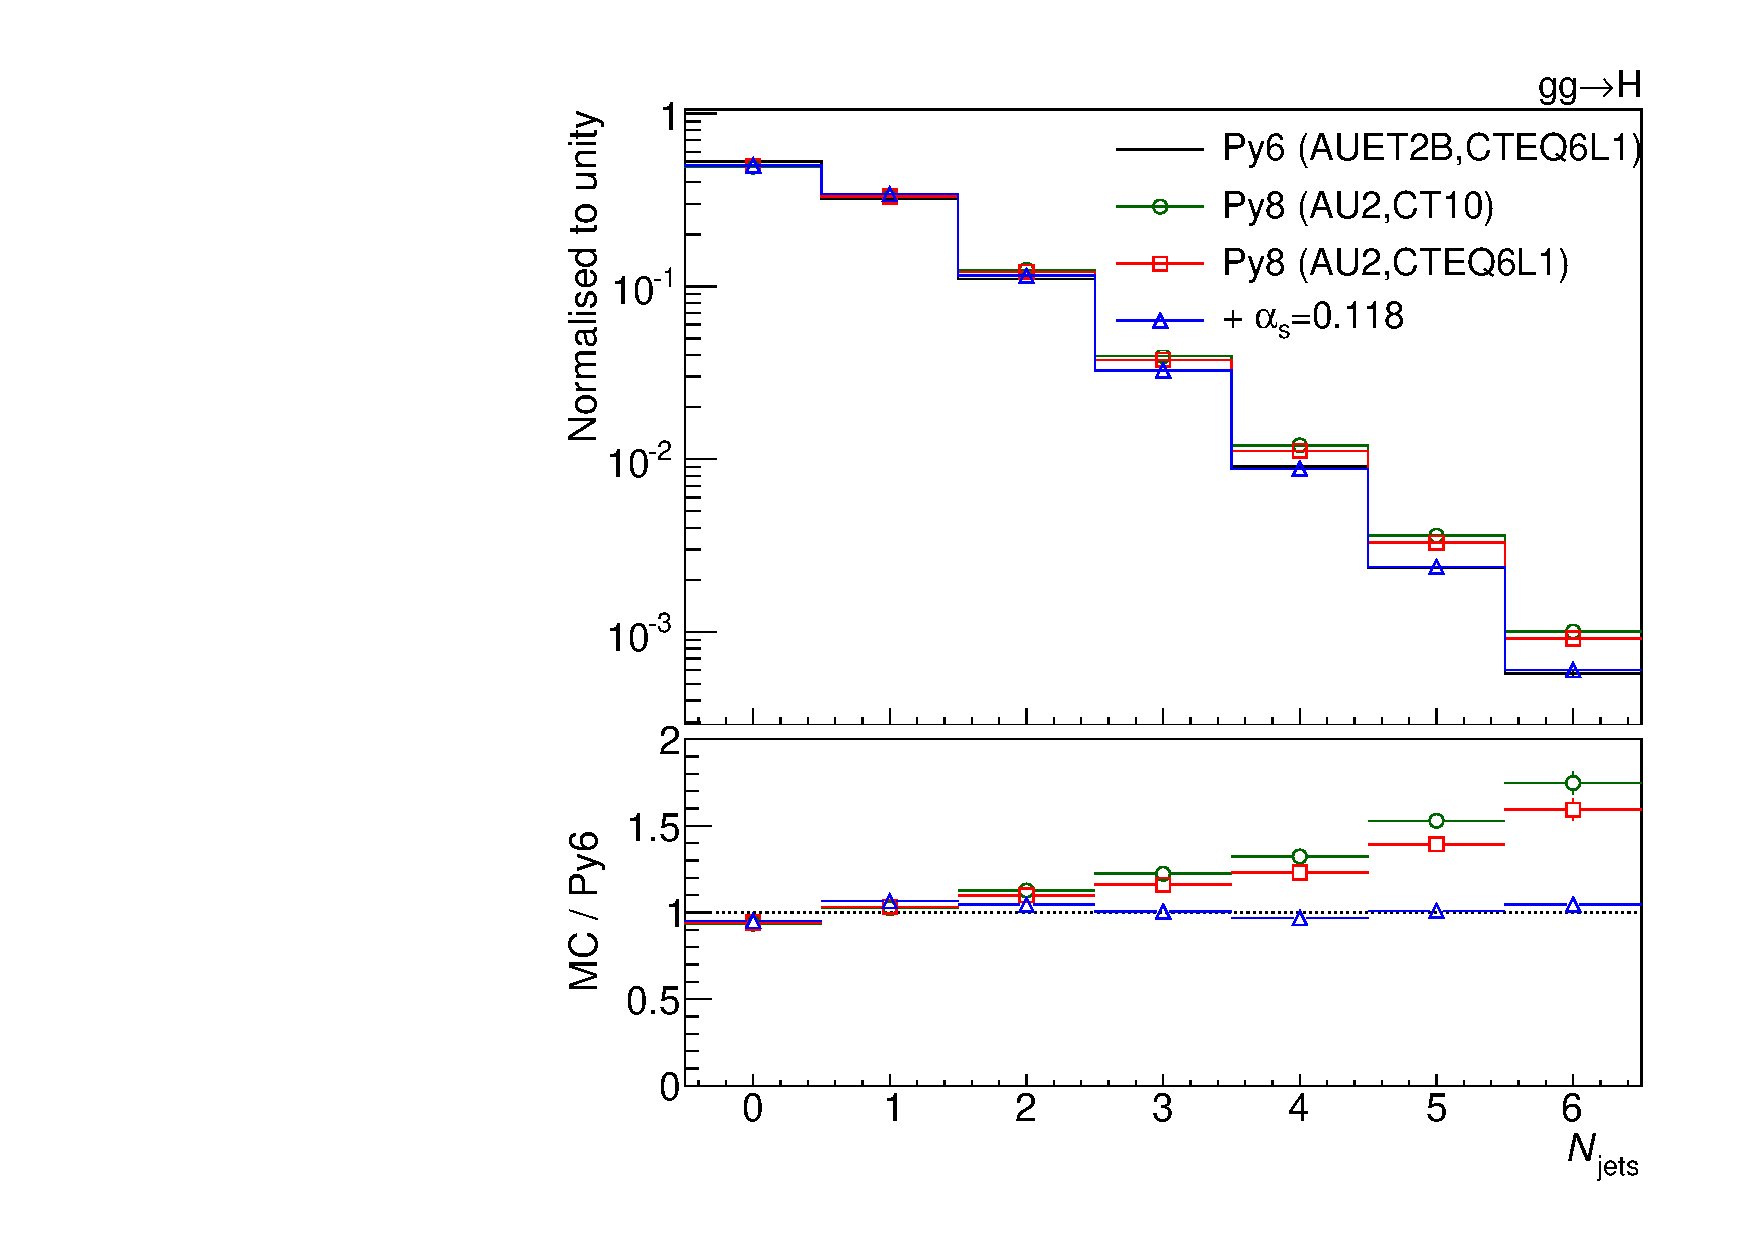
\includegraphics[width=\smallfigwidth]{tex/signal/matching}
	\caption{Jet multiplicity produced by \meps{\powhegbox}{\pythia{8}} with a selection 
	of shower tunes. The green circles is the tune used in the analysis. The red squares 
	change the parton shower PDFs from CT10 to CTEQ6L1. The blue triangles additionally 
	change the parton shower $\alphaS\parenths{\mZ}$ from 0.137 to 0.118 (in agreement 
	with \powhegbox). \meps{\powhegbox}{\pythia{6}} is shown in black for reference.}
	\label{fig:signal:matching}
\end{figure}

Identification of poor matching between \powhegbox and the \pythia{8} parton shower 
program has led to improvements in the latest round of MC tuning \cite{ATLAS:tune:2013}.
